\subsection{Werkzeuge}
Die Entwicklung von Anwendungen für Mikrocontroller bietet eine Reihe von Besonderheiten, insbesondere durch die begrenzte Beobachtbarkeit und Kontrolle zur Laufzeit der Ausführung. Entsprechend müssen auch die genutzten Werkzeuge über spezielle Funktionalitäten verfügen, um die Entwicklung trotzdem effizient zu gestalten. Die in dieser Projektgruppe eingesetzten Tools sollen nun im Folgenden kurz vorgestellt werden.

\subsubsection{Atmel Studio}
Atmel Studio (vormals AVR Studio) ist eine integrierte Entwicklungsumgebung für eingebettete Systeme, insbesondere für die Atmel-eigenen Mikrocontrollerfamilien.
Es basiert auf Microsoft Visual Studio, eignet sich aber insbesondere für die Entwicklung von Software für eingebettete 8- und 32-Bit Controller mit C, C++ und Assembler.
Kern der Anwendung ist ein Cross-Compiler, der es erlaubt, ausführbare Binärdateien direkt für die Zielhardware zu kompilieren.

Abbildung \autoref{fig:avrstudio1} zeigt einen Screenshot vom Atmel Studio. Das Hauptfenster links zeigt die Code-Ansicht mit farblich markierter Code-Struktur, während rechts die Dateistruktur des Projekts abgebildet ist.

\begin{figure}[th]
  \centering
    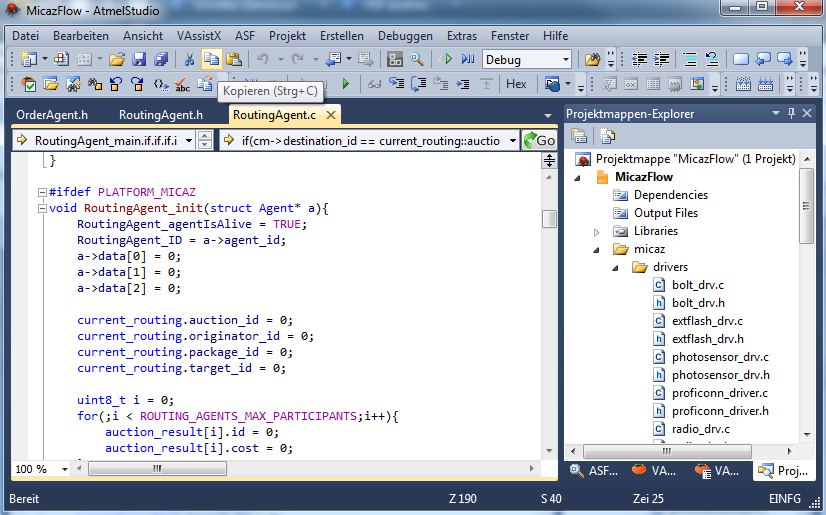
\includegraphics[width = 0.9\textwidth]{flow/AVRStudio_1.png}
    \caption{Entwicklungs-Ansicht des Atmel Studio}
    \label{fig:avrstudio1}
\end{figure}

\begin{figure}[h!]
  \centering
    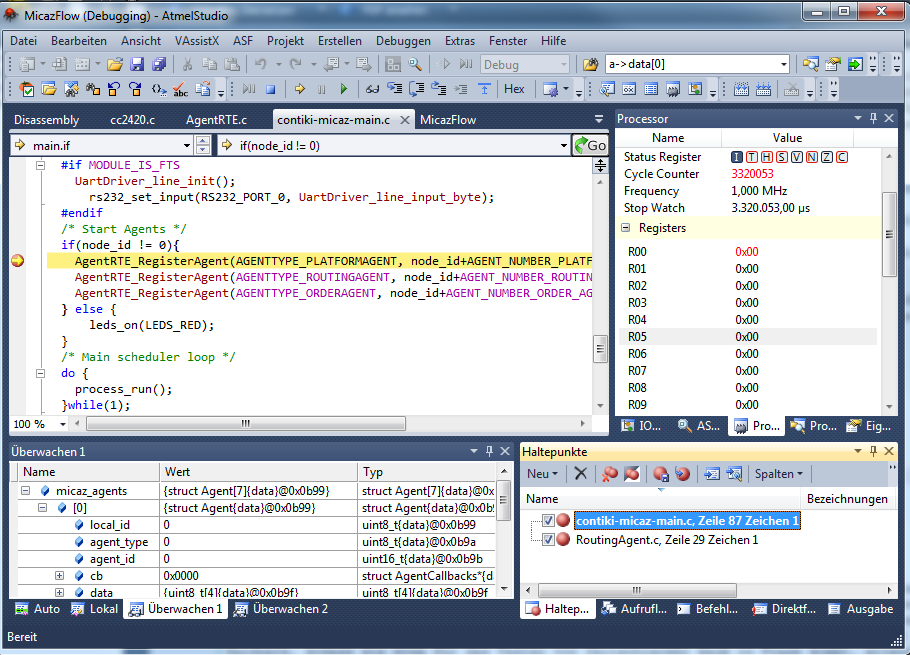
\includegraphics[width = 0.9\textwidth]{flow/AVRStudio_2.png}
    \caption{Debugging-Ansicht des Atmel Studio}
    \label{fig:avrstudio2}
\end{figure}

Neben dem Cross-Compiler beinhaltet das Atmel Studio auch einen Simulator, der es erlaubt, die Ausführung der entwickelten Software auf der Zielhardware zu simulieren. Dabei können Register, Hauptspeicher und Pins des Zielcontrollers beobachtet und Haltepunkte im Code gesetzt werden. Die Simulation ist um ein vielfaches langsamer als die Ausführung auf echter Hardware, sodass sie etwa für das Testen von Zeitschranken kaum in Frage kommt, allerdings gibt sie einen ersten Eindruck von der Funktionalität der eigenen Anwendung.

\subsubsection{AT JTAG ICE3}